% Options for packages loaded elsewhere
\PassOptionsToPackage{unicode}{hyperref}
\PassOptionsToPackage{hyphens}{url}
\PassOptionsToPackage{dvipsnames,svgnames,x11names}{xcolor}
%
\documentclass[
]{article}

\usepackage{amsmath,amssymb}
\usepackage{lmodern}
\usepackage{iftex}
\ifPDFTeX
  \usepackage[T1]{fontenc}
  \usepackage[utf8]{inputenc}
  \usepackage{textcomp} % provide euro and other symbols
\else % if luatex or xetex
  \usepackage{unicode-math}
  \defaultfontfeatures{Scale=MatchLowercase}
  \defaultfontfeatures[\rmfamily]{Ligatures=TeX,Scale=1}
  \setmathfont[]{Latin Modern Math}
\fi
% Use upquote if available, for straight quotes in verbatim environments
\IfFileExists{upquote.sty}{\usepackage{upquote}}{}
\IfFileExists{microtype.sty}{% use microtype if available
  \usepackage[]{microtype}
  \UseMicrotypeSet[protrusion]{basicmath} % disable protrusion for tt fonts
}{}
\makeatletter
\@ifundefined{KOMAClassName}{% if non-KOMA class
  \IfFileExists{parskip.sty}{%
    \usepackage{parskip}
  }{% else
    \setlength{\parindent}{0pt}
    \setlength{\parskip}{6pt plus 2pt minus 1pt}}
}{% if KOMA class
  \KOMAoptions{parskip=half}}
\makeatother
\usepackage{xcolor}
\setlength{\emergencystretch}{3em} % prevent overfull lines
\setcounter{secnumdepth}{5}
% Make \paragraph and \subparagraph free-standing
\ifx\paragraph\undefined\else
  \let\oldparagraph\paragraph
  \renewcommand{\paragraph}[1]{\oldparagraph{#1}\mbox{}}
\fi
\ifx\subparagraph\undefined\else
  \let\oldsubparagraph\subparagraph
  \renewcommand{\subparagraph}[1]{\oldsubparagraph{#1}\mbox{}}
\fi


\providecommand{\tightlist}{%
  \setlength{\itemsep}{0pt}\setlength{\parskip}{0pt}}\usepackage{longtable,booktabs,array}
\usepackage{calc} % for calculating minipage widths
% Correct order of tables after \paragraph or \subparagraph
\usepackage{etoolbox}
\makeatletter
\patchcmd\longtable{\par}{\if@noskipsec\mbox{}\fi\par}{}{}
\makeatother
% Allow footnotes in longtable head/foot
\IfFileExists{footnotehyper.sty}{\usepackage{footnotehyper}}{\usepackage{footnote}}
\makesavenoteenv{longtable}
\usepackage{graphicx}
\makeatletter
\def\maxwidth{\ifdim\Gin@nat@width>\linewidth\linewidth\else\Gin@nat@width\fi}
\def\maxheight{\ifdim\Gin@nat@height>\textheight\textheight\else\Gin@nat@height\fi}
\makeatother
% Scale images if necessary, so that they will not overflow the page
% margins by default, and it is still possible to overwrite the defaults
% using explicit options in \includegraphics[width, height, ...]{}
\setkeys{Gin}{width=\maxwidth,height=\maxheight,keepaspectratio}
% Set default figure placement to htbp
\makeatletter
\def\fps@figure{htbp}
\makeatother
\newlength{\cslhangindent}
\setlength{\cslhangindent}{1.5em}
\newlength{\csllabelwidth}
\setlength{\csllabelwidth}{3em}
\newlength{\cslentryspacingunit} % times entry-spacing
\setlength{\cslentryspacingunit}{\parskip}
\newenvironment{CSLReferences}[2] % #1 hanging-ident, #2 entry spacing
 {% don't indent paragraphs
  \setlength{\parindent}{0pt}
  % turn on hanging indent if param 1 is 1
  \ifodd #1
  \let\oldpar\par
  \def\par{\hangindent=\cslhangindent\oldpar}
  \fi
  % set entry spacing
  \setlength{\parskip}{#2\cslentryspacingunit}
 }%
 {}
\usepackage{calc}
\newcommand{\CSLBlock}[1]{#1\hfill\break}
\newcommand{\CSLLeftMargin}[1]{\parbox[t]{\csllabelwidth}{#1}}
\newcommand{\CSLRightInline}[1]{\parbox[t]{\linewidth - \csllabelwidth}{#1}\break}
\newcommand{\CSLIndent}[1]{\hspace{\cslhangindent}#1}

\usepackage{arxiv}
\usepackage{orcidlink}
\usepackage{amsmath}
\usepackage[T1]{fontenc}
\makeatletter
\makeatother
\makeatletter
\makeatother
\makeatletter
\@ifpackageloaded{caption}{}{\usepackage{caption}}
\AtBeginDocument{%
\ifdefined\contentsname
  \renewcommand*\contentsname{Table of contents}
\else
  \newcommand\contentsname{Table of contents}
\fi
\ifdefined\listfigurename
  \renewcommand*\listfigurename{List of Figures}
\else
  \newcommand\listfigurename{List of Figures}
\fi
\ifdefined\listtablename
  \renewcommand*\listtablename{List of Tables}
\else
  \newcommand\listtablename{List of Tables}
\fi
\ifdefined\figurename
  \renewcommand*\figurename{Figure}
\else
  \newcommand\figurename{Figure}
\fi
\ifdefined\tablename
  \renewcommand*\tablename{Table}
\else
  \newcommand\tablename{Table}
\fi
}
\@ifpackageloaded{float}{}{\usepackage{float}}
\floatstyle{ruled}
\@ifundefined{c@chapter}{\newfloat{codelisting}{h}{lop}}{\newfloat{codelisting}{h}{lop}[chapter]}
\floatname{codelisting}{Listing}
\newcommand*\listoflistings{\listof{codelisting}{List of Listings}}
\makeatother
\makeatletter
\@ifpackageloaded{caption}{}{\usepackage{caption}}
\@ifpackageloaded{subcaption}{}{\usepackage{subcaption}}
\makeatother
\makeatletter
\@ifpackageloaded{tcolorbox}{}{\usepackage[many]{tcolorbox}}
\makeatother
\makeatletter
\@ifundefined{shadecolor}{\definecolor{shadecolor}{rgb}{.97, .97, .97}}
\makeatother
\makeatletter
\makeatother
\ifLuaTeX
  \usepackage{selnolig}  % disable illegal ligatures
\fi
\IfFileExists{bookmark.sty}{\usepackage{bookmark}}{\usepackage{hyperref}}
\IfFileExists{xurl.sty}{\usepackage{xurl}}{} % add URL line breaks if available
\urlstyle{same} % disable monospaced font for URLs
\hypersetup{
  pdftitle={Computational Methods for Drug Repositioning},
  pdfauthor={Rhys McAlister},
  colorlinks=true,
  linkcolor={blue},
  filecolor={Maroon},
  citecolor={Blue},
  urlcolor={Blue},
  pdfcreator={LaTeX via pandoc}}

\renewcommand{\today}{2022-09-19}
\newcommand{\runninghead}{A Preprint }
\title{Computational Methods for Drug Repositioning}
\author{
\textbf{Rhys McAlister}\\}
\date{2022-09-19}
\begin{document}
\maketitle
\ifdefined\Shaded\renewenvironment{Shaded}{\begin{tcolorbox}[enhanced, interior hidden, breakable, boxrule=0pt, sharp corners, borderline west={3pt}{0pt}{shadecolor}, frame hidden]}{\end{tcolorbox}}\fi

\hypertarget{introduction}{%
\section{Introduction}\label{introduction}}

This paper outlines the use of computational chemistry methods to
identify approved drugs that display an inhibitory effect against the
main protease of SARS-CoV-2. This process is known as drug repurposing
but is also termed as drug repositioning or therapeutic switching. This
approach is used to identify novel therapeutic agents from a pool of
existing FDA approved drug molecules. This approach is highly relevant
as the drug discovery process is expensive, time-consuming, and
financially risky. Thus, drug repositioning is employed to increase the
success rate of drug development by offering numerous advantages
relative to tradition drug discovery processes. These include a
substantial reduction in the duration of the drug development process,
lower-cost and higher efficiency and a significantly lower risk of
failure{[}1{]}. The COVID-19 global pandemic highlighted an urgent need
to develop effective therapeutic agents in a much shorter timeframe than
traditional drug discovery processes allow for, thus drug repositioning
efforts have been explored thoroughly as part of the effort to identify
drug molecules for the treatment of COVID-19{[}1{]}. One of the
predominant strategies used in drug-repurposing approaches is the use of
computational methods such as molecular docking or molecular similarity.
Computational methods follow along with the benefits of drug-repurposing
approaches in that they allow for a time and cost efficient approach to
identifying bioactive molecules to be examined for potential use as
pharmacological agents{[}2{]}.

SARS-COV-2 has two proteases: chymotrypsin-like cysteine and main
protease{[}3{]}. These enzymes are responsible for processing
polyproteins which have been translated from viral RNA{[}3{]}.
Inhibition of these proteases would result in an impediment of viral
replication thereby resulting in a therapeutic effect{[}3{]}. It is also
of note that no human proteases are known to share a similar cleavage
specificity thus this inhibitory effect is unlikely to induce a toxic
effect{[}3{]}.

The rise of Omicron subvariants that carry mutations in their spike
proteins leads to concerns regarding the efficacy of neutralising
antibodies and correspondingly the efficacy of existing vaccines and
therapeutic treatments{[}4{]}. Thus, the need for novel and efficacious
chemotherapeutic treatments is clearly apparent. Drug repurposing
efforts powered by computational chemistry methods (virtual
screening/docking studies) provides a systematic path for ongoing drug
discovery efforts to develop therapies effective against SARS-COV-2.

\hypertarget{design}{%
\section{Design}\label{design}}

The authors began by applying a consensus molecular docking protocol to
scan a virtual library of approved drugs (around 2000 drugs). A
high-resolution crystal structure of main protease (Figure 1) that was
co-crystallized with a non-covalent small fragment hit was used as the
basis ligand of this docking study{[}5{]}. This decision was made as the
presence of a ligand within this crystal structure would most likely
alter the conformation of the active site side chain residues in a
manner that would be better for the performance of molecular docking.
The molecular docking protocol of this study included four independent
trials of protein-ligand docking. The docking programs Glide SP,
AutoDock Vina and AutoDock 4.2 were utilised, with AutoDock 4.2 being
used for two of the protocols{[}3{]}. Following this, a ranking of the
compounds in order of their docking scores was conducted and the top 200
hits from each docking trial were compared. From these hits compounds
that were in the top 200 in all four or at least three of the trials
were selected to proceed to the next stage of the experiment. This
docking protocol narrowed the library down to 42 candidates which were
then extensively analyzed with respect to conformation, stability in
molecular dynamics simulations and consideration of intermolecular
contacts. This further narrowed down the candidates to 17, which were
then examined via kinetic assays for inhibition of mPRO.

\begin{figure}[htp]
    \centering
    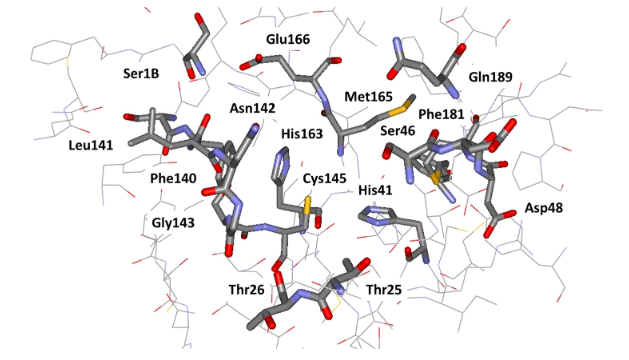
\includegraphics[width=8cm]{Figures/123.PNG}
    \caption{Rendering of the catalytic site of the crystal structure of Main Protease [3]}
    \label{fig:spectra}
\end{figure}

\begin{figure}

{\centering 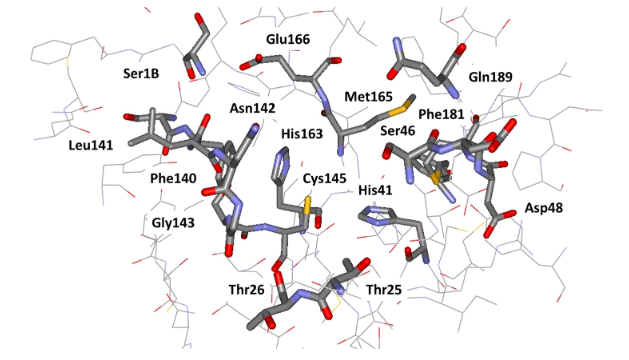
\includegraphics{Figures/123.PNG}

}

\caption{Rendering of the catalytic site of the crystal structure of
Main Protease {[}3{]}}

\end{figure}

\hypertarget{computational-methods}{%
\section{Computational Methods}\label{computational-methods}}

Virtual screening is a computational approach for predicting potentially
bioactive compounds when scanning a library of small molecules {[}2{]}.
The authors of this paper utilised this approach in an attempt to
discover small molecule inhibitors of main protease (mPRO){[}3{]} . They
utilised a form of virtual screening that is receptor based,
specifically they used protein-ligand docking in order to identify drug
molecules that had a potential inhibitory effect on mPRO {[}5{]}.\\

This technique utilises a crystallised structure of a protein in order
to predict how the compounds within the virtual library would bind to
the binding site of a protein{[}2{]}. With this, they analysed more than
50 crystal structures of main protease in both apo and holo forms to
select a structure that would perform optimally in a molecular docking
study. Ultimately selecting a holo crystallised structure of the
SARS-CoV-2 main protease as it was determined that the presence of a
ligand bound to the crystal structure would position the active site
residues in such a manner that would be conducive to optimal performance
of the molecular docking study{[}3{]}.

As part of this technique, the protein used for the basis of docking
must be prepared. As this is an experimentally obtained structure, there
will be aberrations that must be corrected to ensure optimal performance
of the docking protocol {[}6{]}. X-ray crystallographic protein
structures have common issues such as missing hydrogen atoms, missing
residues, incomplete sidechains, undefined protonation states and/or
presence of crystallization products that are not found in
reality{[}2{]}. In order to mitigate these issues the authors of this
paper utilised the program, Reduce, on the crystal structure in order to
perform alterations such as side-chain flips, optimisation of hydrogen
bonds and the addition or removal of hydrogen bonds{[}7{]}. To validate
that this structure was chemically sound, a further program, UCSF
Chimera, was used to visually analyse the structure
{[}{[}5{]}{]}{[}8{]}. The next stage of the virtual screening protocol
was docking. Generally, docking programs generate an initial set of
conformational, tautomeric and protonation states for each of the ligand
compounds{[}5{]}. Then, researchers can apply a search algorithm and
scoring function to generate and score the poses of the ligand within
the binding site of the receptor in an effort to identify the docked
pose that likely represents the real binding mode of the compound
{[}{[}9{]}{]}{[}5{]}. Researchers have the autonomy to introduce
constraints to these processes to assist these protocols in producing
results that make chemical sense. For instance, the cavity of the
protein in which compounds can be docked is commonly constrained in
order to limit the space that can be occupied by docked poses {[}10{]}.
Additionally, constraints regarding the specific binding modes of the
docked poses can be implemented to limit the conformational space the
search algorithm can select docked poses from{[}11{]}.

\begin{figure}[htp]
    \centering
    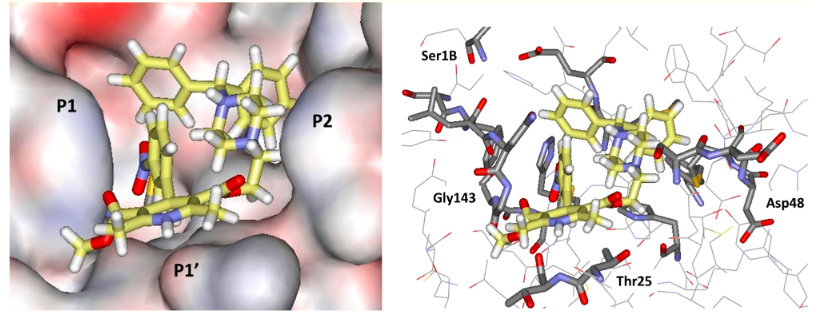
\includegraphics[width=8cm]{Figures/234.png}
    \caption{Glide docking pose of a ligand binding to Main Protease [3]}
    \label{fig:spectra}
\end{figure}

\begin{figure}

{\centering 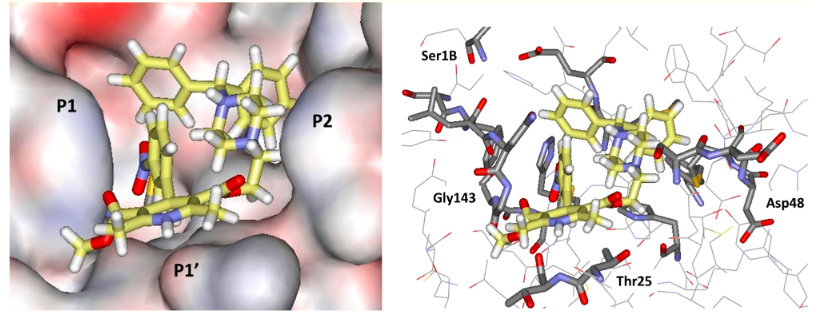
\includegraphics{Figures/234.PNG}

}

\caption{Glide docking pose of a ligand binding to Main Protease
{[}12{]}}

\end{figure}

The authors of this paper ran four independent docking protocols within
this study using Glide SP, AutoDock Vina and two protocols utilising
AutoDock 4.2{[}5{]}. The Glide software package utilises a set of
hierarchical filters to search for probable locations of the ligand
within the binding site region of the receptor {[}13{]}. The receptors
shape and properties are represented using a grid via the use of varying
sets of fields that yield a progressively more accurate scoring of the
ligand pose{[}13{]}. Here, the creators of the Glide software package
define the term `pose' to refer to a complete specification of the
ligand in terms of its position and orientation in space relative to the
receptor, including its core and rotamer group conformations {[}13{]}.
Following the field generation, generation of initial ligand
conformations is performed. This set of conformations are selected from
a listing of the minima energy structures within the ligand dihedral
angle space {[}13{]}. Utilising these generated conformations, an
initial screening procedure is performed to identify promising poses,
this pre-screening step reduces the region where more computationally
expensive evaluations are performed thereby allowing for acceptable
computational speed{[}13{]}. Beginning with the promising poses
identified from this initial screening, the ligands are the minimised
within the field of the receptor via the use of a standard molecular
mechanics energy function in order to select for a smaller sub-selection
of low energy poses {[}13{]}. To finally predict the binding affinity
and order the screened ligands, a combination of `GlideScore', the
ligand-receptor molecular mechanics energy and the ligand strain energy
is utilised in order to identify correctly docked poses {[}13{]}.

\hypertarget{section}{%
\section*{}\label{section}}
\addcontentsline{toc}{section}{}

\hypertarget{refs}{}
\begin{CSLReferences}{0}{0}
\leavevmode\vadjust pre{\hypertarget{ref-10.3389ux2ffmolb.2021.628144}{}}%
\CSLLeftMargin{{[}1{]} }%
\CSLRightInline{B.M. Sahoo, B.V.V. Ravi Kumar, J. Sruti, M.K. Mahapatra,
B.K. Banik, P. Borah, Drug repurposing strategy (DRS): Emerging approach
to identify potential therapeutics for treatment of novel coronavirus
infection, Frontiers in Molecular Biosciences. 8 (2021).
https://doi.org/\href{https://doi.org/10.3389/fmolb.2021.628144}{10.3389/fmolb.2021.628144}.}

\leavevmode\vadjust pre{\hypertarget{ref-gimeno2019}{}}%
\CSLLeftMargin{{[}2{]} }%
\CSLRightInline{A. Gimeno, M. Ojeda-Montes, S. Tomás-Hernández, A.
Cereto-Massagué, R. Beltrán-Debón, M. Mulero, G. Pujadas, S.
Garcia-Vallvé, The light and dark sides of virtual screening: What is
there to know?, International Journal of Molecular Sciences. 20 (2019)
1375.
https://doi.org/\href{https://doi.org/10.3390/ijms20061375}{10.3390/ijms20061375}.}

\leavevmode\vadjust pre{\hypertarget{ref-jin2020}{}}%
\CSLLeftMargin{{[}3{]} }%
\CSLRightInline{Z. Jin, X. Du, Y. Xu, Y. Deng, M. Liu, Y. Zhao, B.
Zhang, X. Li, L. Zhang, C. Peng, Y. Duan, J. Yu, L. Wang, K. Yang, F.
Liu, R. Jiang, X. Yang, T. You, X. Liu, X. Yang, F. Bai, H. Liu, X. Liu,
L.W. Guddat, W. Xu, G. Xiao, C. Qin, Z. Shi, H. Jiang, Z. Rao, H. Yang,
Structure of mpro from SARS-CoV-2 and discovery of its inhibitors,
Nature. 582 (2020) 289--293.
https://doi.org/\href{https://doi.org/10.1038/s41586-020-2223-y}{10.1038/s41586-020-2223-y}.}

\leavevmode\vadjust pre{\hypertarget{ref-wang2022}{}}%
\CSLLeftMargin{{[}4{]} }%
\CSLRightInline{Q. Wang, Y. Guo, S. Iketani, M.S. Nair, Z. Li, H. Mohri,
M. Wang, J. Yu, A.D. Bowen, J.Y. Chang, J.G. Shah, N. Nguyen, Z. Chen,
K. Meyers, M.T. Yin, M.E. Sobieszczyk, Z. Sheng, Y. Huang, L. Liu, D.D.
Ho, Antibody evasion by SARS-CoV-2 omicron subvariants BA.2.12.1, BA.4
and BA.5, Nature. 608 (2022) 603--608.
https://doi.org/\href{https://doi.org/10.1038/s41586-022-05053-w}{10.1038/s41586-022-05053-w}.}

\leavevmode\vadjust pre{\hypertarget{ref-ghahremanpour2020}{}}%
\CSLLeftMargin{{[}5{]} }%
\CSLRightInline{M.M. Ghahremanpour, J. Tirado-Rives, M. Deshmukh, J.A.
Ippolito, C.-H. Zhang, I. Cabeza De Vaca, M.-E. Liosi, K.S. Anderson,
W.L. Jorgensen, Identification of 14 known drugs as inhibitors of the
main protease of SARS-CoV-2, ACS Medicinal Chemistry Letters. 11 (2020)
2526--2533.
https://doi.org/\href{https://doi.org/10.1021/acsmedchemlett.0c00521}{10.1021/acsmedchemlett.0c00521}.}

\leavevmode\vadjust pre{\hypertarget{ref-gimeno2019c}{}}%
\CSLLeftMargin{{[}6{]} }%
\CSLRightInline{A. Gimeno, M. Ojeda-Montes, S. Tomás-Hernández, A.
Cereto-Massagué, R. Beltrán-Debón, M. Mulero, G. Pujadas, S.
Garcia-Vallvé, The light and dark sides of virtual screening: What is
there to know?, International Journal of Molecular Sciences. 20 (2019)
1375.
https://doi.org/\href{https://doi.org/10.3390/ijms20061375}{10.3390/ijms20061375}.}

\leavevmode\vadjust pre{\hypertarget{ref-ghahremanpour2020b}{}}%
\CSLLeftMargin{{[}7{]} }%
\CSLRightInline{M.M. Ghahremanpour, J. Tirado-Rives, M. Deshmukh, J.A.
Ippolito, C.-H. Zhang, I. Cabeza De Vaca, M.-E. Liosi, K.S. Anderson,
W.L. Jorgensen, Identification of 14 known drugs as inhibitors of the
main protease of SARS-CoV-2, ACS Medicinal Chemistry Letters. 11 (2020)
2526--2533.
https://doi.org/\href{https://doi.org/10.1021/acsmedchemlett.0c00521}{10.1021/acsmedchemlett.0c00521}.}

\leavevmode\vadjust pre{\hypertarget{ref-pettersen2004a}{}}%
\CSLLeftMargin{{[}8{]} }%
\CSLRightInline{E.F. Pettersen, T.D. Goddard, C.C. Huang, G.S. Couch,
D.M. Greenblatt, E.C. Meng, T.E. Ferrin, UCSF chimera?a visualization
system for exploratory research and analysis, Journal of Computational
Chemistry. 25 (2004) 1605--1612.
https://doi.org/\href{https://doi.org/10.1002/jcc.20084}{10.1002/jcc.20084}.}

\leavevmode\vadjust pre{\hypertarget{ref-pettersen2004}{}}%
\CSLLeftMargin{{[}9{]} }%
\CSLRightInline{E.F. Pettersen, T.D. Goddard, C.C. Huang, G.S. Couch,
D.M. Greenblatt, E.C. Meng, T.E. Ferrin, UCSF chimera?a visualization
system for exploratory research and analysis, Journal of Computational
Chemistry. 25 (2004) 1605--1612.
https://doi.org/\href{https://doi.org/10.1002/jcc.20084}{10.1002/jcc.20084}.}

\leavevmode\vadjust pre{\hypertarget{ref-gimeno2019a}{}}%
\CSLLeftMargin{{[}10{]} }%
\CSLRightInline{A. Gimeno, M. Ojeda-Montes, S. Tomás-Hernández, A.
Cereto-Massagué, R. Beltrán-Debón, M. Mulero, G. Pujadas, S.
Garcia-Vallvé, The light and dark sides of virtual screening: What is
there to know?, International Journal of Molecular Sciences. 20 (2019)
1375.
https://doi.org/\href{https://doi.org/10.3390/ijms20061375}{10.3390/ijms20061375}.}

\leavevmode\vadjust pre{\hypertarget{ref-gimeno2019b}{}}%
\CSLLeftMargin{{[}11{]} }%
\CSLRightInline{A. Gimeno, M. Ojeda-Montes, S. Tomás-Hernández, A.
Cereto-Massagué, R. Beltrán-Debón, M. Mulero, G. Pujadas, S.
Garcia-Vallvé, The light and dark sides of virtual screening: What is
there to know?, International Journal of Molecular Sciences. 20 (2019)
1375.
https://doi.org/\href{https://doi.org/10.3390/ijms20061375}{10.3390/ijms20061375}.}

\leavevmode\vadjust pre{\hypertarget{ref-ghahremanpour2020a}{}}%
\CSLLeftMargin{{[}12{]} }%
\CSLRightInline{M.M. Ghahremanpour, J. Tirado-Rives, M. Deshmukh, J.A.
Ippolito, C.-H. Zhang, I. Cabeza De Vaca, M.-E. Liosi, K.S. Anderson,
W.L. Jorgensen, Identification of 14 known drugs as inhibitors of the
main protease of SARS-CoV-2, ACS Medicinal Chemistry Letters. 11 (2020)
2526--2533.
https://doi.org/\href{https://doi.org/10.1021/acsmedchemlett.0c00521}{10.1021/acsmedchemlett.0c00521}.}

\leavevmode\vadjust pre{\hypertarget{ref-friesner2004}{}}%
\CSLLeftMargin{{[}13{]} }%
\CSLRightInline{R.A. Friesner, J.L. Banks, R.B. Murphy, T.A. Halgren,
J.J. Klicic, D.T. Mainz, M.P. Repasky, E.H. Knoll, M. Shelley, J.K.
Perry, D.E. Shaw, P. Francis, P.S. Shenkin, Glide:{\hspace{0.167em}} A
new approach for rapid, accurate docking and scoring. 1. Method and
assessment of docking accuracy, Journal of Medicinal Chemistry. 47
(2004) 1739--1749.
https://doi.org/\href{https://doi.org/10.1021/jm0306430}{10.1021/jm0306430}.}

\end{CSLReferences}



\end{document}
